%\begin{appendices}

\appendix
%\chapter*{ANEXOS}% If \appendix doesn't insert a \chapter
%\addcontentsline{toc}{chapter}{ANEXOS}% Print Appendix in ToC
\setcounter{section}{0}% Reset numbering for sections
\renewcommand{\thesection}{\Alph{section}}% Adjust section printing (from here onward)
	
	\section{Árbol de Problemas}
	%\chapter*{Árbol de Problemas}
	%\addcontentsline{toc}{section}{Árbol de Problemas}
	%\renewcommand{\thechapter}{A}
	\label{anexo1}
	\begin{figure}[h]
		\begin{center}
			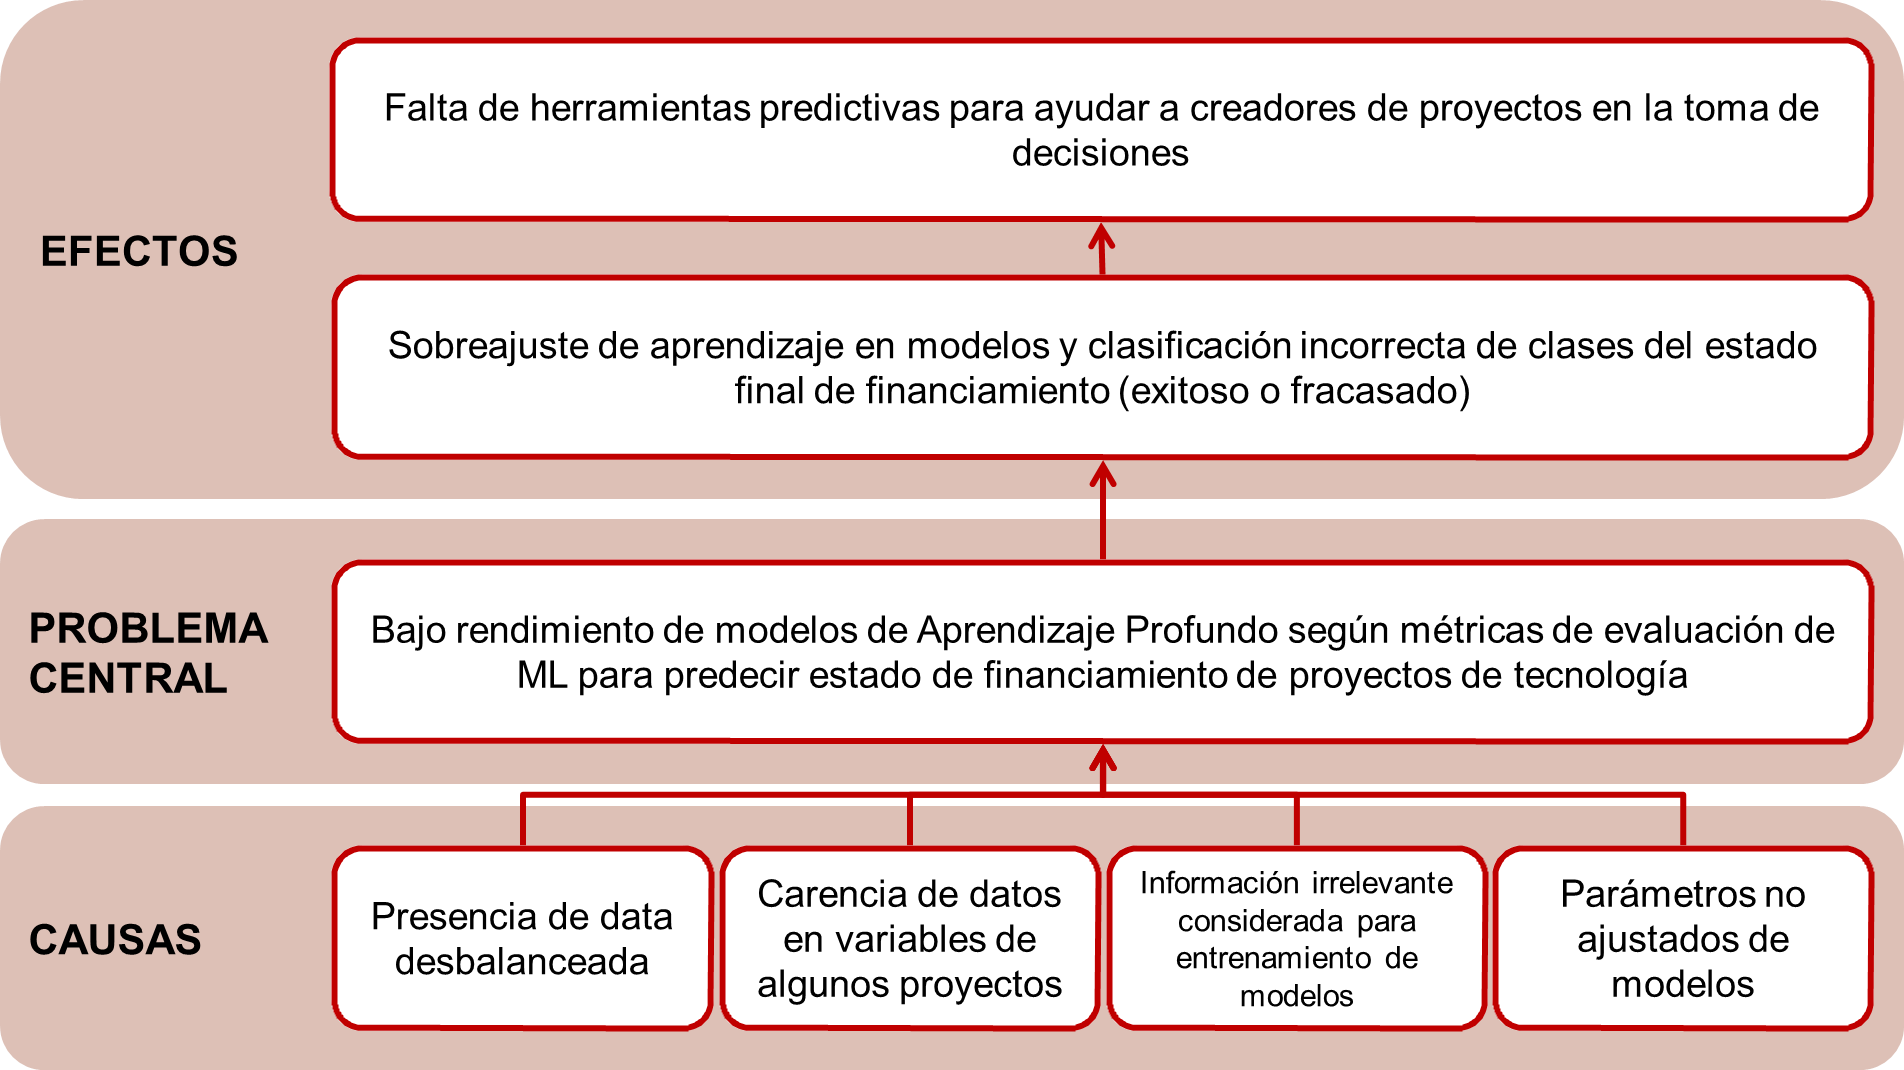
\includegraphics[width=1.05\textwidth]{anexos/arbol_problemas.png}
			%\caption{Fuente: Elaboración propia}
		\end{center}
	\end{figure}
	\clearpage
	
	\section{Árbol de Objetivos}
	%\chapter*{Árbol de Objetivos}
	%\addcontentsline{toc}{section}{Árbol de Objetivos}
	%\renewcommand{\thechapter}{A}
	\label{anexo2}
	\begin{figure}[h]
		\begin{center}
			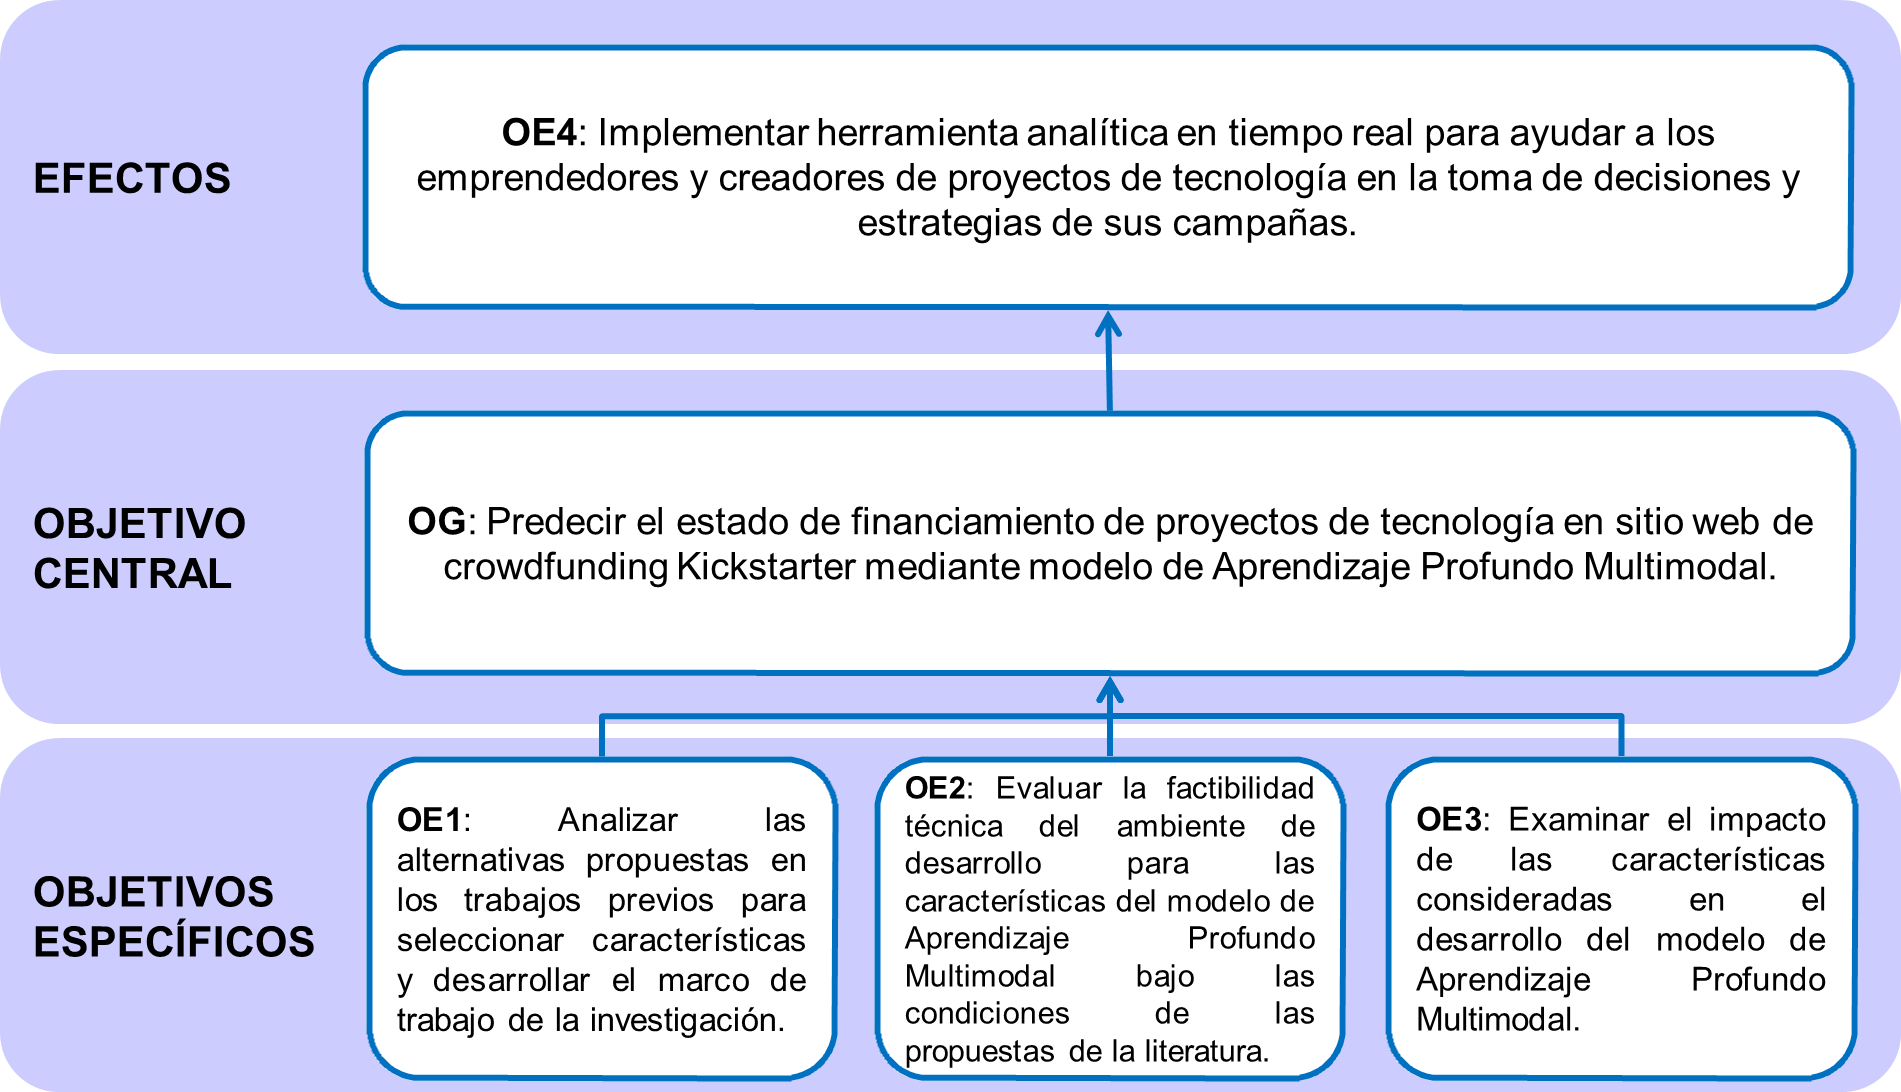
\includegraphics[width=1.05\textwidth]{anexos/arbol_objetivos.png}
			%\caption{Fuente: Elaboración propia}
		\end{center}
	\end{figure}
	\clearpage
	
	\begin{landscape}
		\section{Matriz de Consistencia}
		\label{anexo3}
		\begin{longtable}{ p{3.5cm}p{3.5cm}p{3.5cm}p{3cm}p{3cm}p{3cm}p{3cm} }
			%\centering
			\small
			\tabularnewline \specialrule{.1em}{.05em}{.05em}
			\centering{Título de la tesis} & \multicolumn{6}{p{19cm}}{Predicción del estado de financiamiento de proyectos de tecnología en sitio web de crowdfunding Kickstarter mediante modelo de Aprendizaje Profundo Multimodal}
			\tabularnewline \specialrule{.1em}{.05em}{.05em}
			\Centering{Problema General}& \Centering{Objetivo General}& \Centering{Hipótesis General}& \Centering{Variables}& \Centering{Dimensiones}& \Centering{Indicadores}& \Centering{Metodología}
			\\
			\specialrule{.1em}{.05em}{.05em}
			{\ProblemaGeneral} & { \ObjetivoGeneral} & {\HipotesisGeneral}
			& \multirow{3}{3cm}[-28ex]{
				\centering Independiente: Aprendizaje Profundo Multimodal
			}
			& \multirow{2}{3cm}[-30ex]{
				\centering Modelo de Aprendizaje Profundo
			}
			& \multirow{1}{3cm}[-10ex]{
				\centering Cantidad de modelos de Aprendizaje Profundo
			}
			& \multirow{2}{3cm}[3ex]{
			\setlist{nolistsep}
			\begin{itemize}[label={--},nosep,noitemsep,leftmargin=*,topsep=0pt,partopsep=0pt]
				\item Tipo de investigación: Diseño Experimental.
				\item Alcance de la investigación: Descriptivo, porque busca describir las características de un fenómeno.
				\item Enfoque de investigación: Cuantitativa.
			\end{itemize}
			}
			\\
			\cline{1-3}
			\cline{6-6}
			\Centering{Problemas Específicos}& \Centering{Objetivos Específicos} & \Centering{Hipótesis Específicas}
			& 
			&
			& \multirow{1}{3cm}[-10ex]{
				\centering Efectividad de modelos de Aprendizaje Profundo
			}
			& 
			\\
			\cline{1-3}
			\vspace{0pt}{\Pbone} & \vspace{0pt}{\Objone} & \vspace{0pt}{\Hone} &  &  &  &
			\\
			\cline{1-3}
			\cline{5-6}
			\vspace{0pt}{\Pbtwo} & \vspace{0pt}{\Objtwo} & \vspace{0pt}{\Htwo} &  & \multirow{2}{3cm}[-15ex]{
				\centering Estructura del modelo de Aprendizaje Profundo
			} & \multirow{1}{3cm}[-13ex]{
				\centering Complejidad de la estructura de modelos de Aprendizaje Profundo
			} &
			\\
			\cline{1-6}
			\vspace{0pt}{\Pbthree} & \vspace{0pt}{\Objthree} & \vspace{0pt}{\Hthree}
			& \multirow{2}{3cm}[-20ex]{
				\centering Dependiente: Financiamiento de un proyecto
			} 
			& \multirow{1}{3cm}[-10ex]{
				\centering Crowdfunding
			}
			& \multirow{1}{3cm}[-6.5ex]{
				\centering Estado de financiamiento de un proyecto
			}
			& 
			\\
			\cline{1-3}
			\cline{5-6}
			\vspace{0pt}{\Pbfour} & \vspace{0pt}{\Objfour} & \vspace{0pt}{\Hfour} &  & \multirow{1}{3cm}[-12ex]{
				\centering Campaña del proyecto en Kickstarter
			} & \multirow{1}{3.5cm}[-8ex]{
				\setlist{nolistsep}
				\begin{itemize}[label={--},nosep,noitemsep,leftmargin=*,topsep=0pt,partopsep=0pt]
					\item Metainformación.
					\item Descripción.
					\item Comentarios.
				\end{itemize}
			} &
			\\
			\specialrule{.1em}{.05em}{.05em}
		\end{longtable}
	\end{landscape}
	\clearpage
	
	\section{Comparación de metodologías de antecedentes}
	%\chapter{Comparación de metodologías de antecedentes}
	%\addcontentsline{toc}{section}{Comparación de metodologías de antecedentes}
	\label{anexo4}
	%\begin{table}[htbp]
	\begingroup
		\renewcommand\arraystretch{0.5}
		\begin{longtable}{M{3cm}M{5.5cm}M{5.5cm}M{1.5cm}}
			\centering
			\small
			%% Se agrega tabularnewline para longtable
			\tabularnewline \specialrule{.1em}{.05em}{.05em}
			Autor & Título de la Investigación & Metodología & Grupo
			\\
			\specialrule{.1em}{.05em}{.05em}
			Chen, Jones, Kim \& Schlamp
			& KickPredict: Predicting Kickstarter Success
			& \setlist{nolistsep}
			\begin{itemize}[label={--},nosep,noitemsep,leftmargin=*,topsep=0pt,partopsep=0pt]
				\item Recolección de datos.
				\item Modelamiento.
				\item Evaluación.
				\item Despliegue.
			\end{itemize}
			& GG
			\\
			\hline
			Mitra \& Gilbert
			& The Language that Gets People to Give: Phrases that Predict Success on Kickstarter
			& \setlist{nolistsep}
			\begin{itemize}[label={--},nosep,noitemsep,leftmargin=*,topsep=0pt,partopsep=0pt]
				\item Recolección de datos.
				\item Pre-procesamiento de datos.
				\item Modelamiento.
				\item Evaluación.
				\item Despliegue.
			\end{itemize}
			& GE
			\\
			\hline
			Zhou, Zhang, Wang, Du, Qiao \& Fan
			& Money Talks: A Predictive Model on Crowdfunding Success Using Project Description
			& \setlist{nolistsep}
			\begin{itemize}[label={--},nosep,noitemsep,leftmargin=*,topsep=0pt,partopsep=0pt]
				\item Formulación del problema.
				\item Recolección de datos.
				\item Pre-procesamiento de datos.
				\item Modemiento.
				\item Evaluación.
			\end{itemize}
			& GD
			\\
			\hline
			Chen, Chen, Chen, Yang, Lin \& Wei
			& Will Your Project Get the Green Light? Predicting the Success of Crowdfunding Campaigns
			& \setlist{nolistsep}
			\begin{itemize}[label={--},nosep,noitemsep,leftmargin=*,topsep=0pt,partopsep=0pt]
				\item Recolección de datos.
				\item Pre-procesamiento de datos.
				\item Modelamiento.
				\item Evaluación.
			\end{itemize}
			& GF
			\\
			\hline
			Beckwith
			& Predicting Success in Equity Crowdfunding
			& \setlist{nolistsep}
			\begin{itemize}[label={--},nosep,noitemsep,leftmargin=*,topsep=0pt,partopsep=0pt]
				\item Recolección de datos.
				\item Pre-procesamiento de datos.
				\item Modelamiento.
				\item Evaluación.
			\end{itemize}
			&  GF
			\\
			\hline
			Li, Rakesh \& Reddy
			& Project Success Prediction in Crowdfunding Environments
			& \setlist{nolistsep}
			\begin{itemize}[label={--},nosep,noitemsep,leftmargin=*,topsep=0pt,partopsep=0pt]
				\item Formulación del problema.
				\item Recolección de datos.
				\item Pre-procesamiento de datos.
				\item Modelamiento.
				\item Evaluación.
			\end{itemize}
			& GD
			\\
			\hline
			Yuan, Lau \& Xu
			& The Determinants of Crowdfunding Success: A Semantic Text Analytics Approach
			& \setlist{nolistsep}
			\begin{itemize}[label={--},nosep,noitemsep,leftmargin=*,topsep=0pt,partopsep=0pt]
				\item Recolección de datos.
				\item Pre-procesamiento de datos.
				\item Modelamiento.
				\item Evaluación.
				\item Despliegue.
			\end{itemize}
			& GE
			\\
			\hline
			Sawhney, Tran \& Tuason
			& Using Language to Predict Kickstarter Success
			& \setlist{nolistsep}
			\begin{itemize}[label={--},nosep,noitemsep,leftmargin=*,topsep=0pt,partopsep=0pt]
				\item Recolección de datos.
				\item Modelamiento.
				\item Evaluación.
			\end{itemize}
			& GH
			\\
			\hline
			Kaur \& Gera
			& Effect of Social Media Connectivity on Success of Crowdfunding Campaigns
			& \setlist{nolistsep}
			\begin{itemize}[label={--},nosep,noitemsep,leftmargin=*,topsep=0pt,partopsep=0pt]
				\item Recolección de datos.
				\item Pre-procesamiento de datos.
				\item Modelamiento.
				\item Evaluación.
			\end{itemize}
			& GF
			\\
			\hline
			Kamath \& Kamat
			& Supervised Learning Model For Kickstarter Campaigns With R Mining
			& \setlist{nolistsep}
			\begin{itemize}[label={--},nosep,noitemsep,leftmargin=*,topsep=0pt,partopsep=0pt]
				\item Formulación del problema.
				\item Recolección y pre-procesamiento de datos.
				\item Exploración y extracción de datos.
				\item Modelamiento.
				\item Evaluación.
			\end{itemize}
			& GD
			\\
			\hline
			Yu, Huang, Yang, Liu, Li \& Tsai
			& Prediction of Crowdfunding Project Success with Deep Learning
			& \setlist{nolistsep}
			\begin{itemize}[label={--},nosep,noitemsep,leftmargin=*,topsep=0pt,partopsep=0pt]
				\item Recolección de datos.
				\item Exploración de datos.
				\item Pre-procesamiento de datos.
				\item Modelamiento.
				\item Evaluación.
			\end{itemize}
			& GE
			\\
			\hline
			Lee, Lee \& Kim
			& Content-based Success Prediction of Crowdfunding Campaigns: A Deep Learning Approach
			& \setlist{nolistsep}
			\begin{itemize}[label={--},nosep,noitemsep,leftmargin=*,topsep=0pt,partopsep=0pt]
				\item Recolección de datos.
				\item Modelamiento.
				\item Evaluación.
			\end{itemize}
			& GH
			\\
			\hline
			Jin, Zhao, Chen, Liu \& Ge
			& Estimating the Days to Success of Campaigns in Crowdfunding: A Deep Survival Perspective
			& \setlist{nolistsep}
			\begin{itemize}[label={--},nosep,noitemsep,leftmargin=*,topsep=0pt,partopsep=0pt]
				\item Formulación del problema.
				\item Recolección de datos.
				\item Pre-procesamiento de datos.
				\item Modelamiento.
				\item Evaluación.
				\item Despliegue.
			\end{itemize}
			& GA
			\\
			\hline
			Cheng, Tan, Hou \& Wei
			& Success Prediction on Crowdfunding with Multimodal Deep Learning
			& \setlist{nolistsep}
			\begin{itemize}[label={--},nosep,noitemsep,leftmargin=*,topsep=0pt,partopsep=0pt]
				\item Formulación del problema.
				\item Recolección de datos.
				\item Pre-procesamiento de datos.
				\item Modelamiento.
				\item Evaluación.
				\item Despliegue.
			\end{itemize}
			& GA
			\\
			\hline
			Chen \& Shen
			& Finding the Keywords Affecting the Success of Crowdfunding Projects
			& \setlist{nolistsep}
			\begin{itemize}[label={--},nosep,noitemsep,leftmargin=*,topsep=0pt,partopsep=0pt]
				\item Recolección de datos.
				\item Pre-procesamiento de datos.
				\item Selección de características.
				\item Modelamiento.
				\item Evaluación.
			\end{itemize}
			& GC
			\\
			\hline
			Chaichi \& Anderson
			& Deploying Natural Language Processing to Extract Key Product Features of Crowdfunding Campaigns: The Case of 3D Printing Technologies on Kickstarter
			& \setlist{nolistsep}
			\begin{itemize}[label={--},nosep,noitemsep,leftmargin=*,topsep=0pt,partopsep=0pt]
				\item Recolección de datos.
				\item Pre-procesamiento de datos.
				\item Selección de características.
				\item Modelamiento.
				\item Evaluación.
			\end{itemize}
			& GC
			\\
			\hline
			Shafqat \& Byun
			& Topic Predictions and Optimized Recommendation Mechanism Based on Integrated Topic Modeling and Deep Neural Networks in Crowdfunding Platforms
			& \setlist{nolistsep}
			\begin{itemize}[label={--},nosep,noitemsep,leftmargin=*,topsep=0pt,partopsep=0pt]
				\item Formulación del problema.
				\item Recolección de datos.
				\item Selección de características.
				\item Modelamiento.
				\item Evaluación.
				\item Despliegue.
			\end{itemize}
			& GB
			\\
			\hline
			Fernández-Blanco, Villanueva-Balsera, Rodriguez-Montequin \& Moran-Palacios
			& Key Factors for Project Crowdfunding Success: An Empirical Study
			& \setlist{nolistsep}
			\begin{itemize}[label={--},nosep,noitemsep,leftmargin=*,topsep=0pt,partopsep=0pt]
				\item Entendimiento del problema.
				\item Entendimiento de los datos.
				\item Preparación de los datos.
				\item Modelamiento.
				\item Evaluación.
				\item Despliegue.
			\end{itemize}
			& CRISP-DM
			\\
			\specialrule{.1em}{.05em}{.05em}
		\end{longtable}%
	\endgroup
	%\end{table}
	\clearpage
	
	\begin{landscape}
		\section{Comparación de objetivos específicos de antecedentes}
		\label{anexo5}
		\begin{longtable}{M{1cm}m{2.8cm}m{2.8cm}m{4.4cm}m{4cm}m{6cm}M{1cm}}
			\newcommand{\multirot}[1]{\multirow{2}{*}[-8ex]{\rotcell{\rlap{#1}}}}
			%\scriptsize
			\footnotesize
			\centering
			\tabularnewline \specialrule{.1em}{.05em}{.05em}
			\centering Año & \centering Autor & \centering Publicación & \centering Título de la Investigación & \centering Objetivo General & \centering Objetivos Específicos & \centering Item
			\\%%[5pt]
			\tabularnewline \specialrule{.1em}{.05em}{.05em}
			\multirow{3}{1cm}[-9ex]{\centering 2013} & \multirow{3}{2.8cm}[-9ex]{Chen, Jones, Kim, Schlamp} & \multirow{3}{2.8cm}[-9ex]{Reporte técnico} & \multirow{3}{4.4cm}[-9ex]{KickPredict: Predicting Kickstarter Success} & \multirow{3}{4cm}[-3ex]{Desarrollar un sistema para predecir si un proyecto de Kickstarter será financiado exitosamente o no antes de su culminación.} & {Desarrollar aplicaciones en Android y Google Chrome para predecir en tiempo real el estado de financiamiento y el porcentaje.} & {OE4}
			\\%%[10pt]
			\cline{6-7}
			 &  &  &  &  & {Analizar las características más importantes que influyen en el éxito de financiamiento a partir de las propiedades de los proyectos.} & {OE3}
			\\%%[10pt]
			\cline{6-7}
			 &  &  &  &  & {Estudiar el impacto de contribuciones durante el transcurso de la campaña en el estado de financiamiento.} & 
			\\
			\hline
			\multirow{2}{1cm}[-4ex]{\centering 2014} & \multirow{2}{2.8cm}[-4ex]{Mitra, Gilbert} & \multirow{2}{2.8cm}[-4ex]{Acta de conferencia} & \multirow{2}{4.4cm}[-1ex]{The Language that Gets People to Give: Phrases that Predict Success on Kickstarter} & \multirow{2}{4cm}[1ex]{Determinar los factores que conducen a financiar con éxito un proyecto de crowdfunding.} & {Desarrollar frases predictivas junto con variables de control para ayudar a posteriores estudios y creadores de proyectos.} & {OE4}
			\\
			\cline{6-7}
			&  &  &  &  & {Evaluar el impacto del uso de ciertas frases de la descripción en el éxito de financiamiento.} & {OE3}
			\\
			\hline
			\multirow{2}{1cm}[-4ex]{\centering 2015} & \multirow{2}{2.8cm}[-2ex]{Zhou, Zhang, Wang, Du, Qiao, Fan} & \multirow{2}{2.8cm}[-4ex]{Acta de conferencia} & \multirow{2}{4.4cm}[2ex]{Money Talks: A Predictive Model on Crowdfunding Success Using Project Description} & \multirow{2}{4cm}[3ex]{Estudiar la influencia de las descripciones de proyectos en el éxito de financiamiento de proyectos crowdfunding.} & {Examinar el impacto de la calidad argumentativa y fuente de credibilidad de la descripción de un proyecto en su performance durante la campaña.} & {OE3}
			\\
			\cline{6-7}
			&  &  &  &  & {Evaluar e implementar características previamente consideradas en trabajos previos.} & {OE1}
			\\
			\hline
			\multirow{3}{1cm}[-3ex]{\centering 2015} & \multirow{3}{2.8cm}[-3ex]{Chen, Chen, Chen, Yang, Lin, Wei} & \multirow{3}{2.8cm}[-3ex]{Acta de conferencia} & \multirow{3}{4.4cm}[0ex]{Will Your Project Get the Green Light? Predicting the Success of Crowdfunding Campaigns} & \multirow{3}{4cm}[3ex]{Predecir si una campaña de crowdfunding tendrá éxito a través de extracción y posterior uso de características estáticas y dinámicas.} & {Analizar relación entre exactitud del modelo y el uso de características dinámicas y/o estáticas.} & {OE3}
			\\%%[10pt]
			\cline{6-7}
			&  &  &  &  & {Evaluar efectividad de predicción en distintas etapas de campaña.} & {}
			\\%%[10pt]
			\cline{6-7}
			&  &  &  &  & {Evaluar características estáticas y dinámicas de trabajos previos.} & {OE1}
			\\
			\hline
			\multirow{2}{1cm}[-5ex]{\centering 2016} & \multirow{2}{2.8cm}[-5ex]{Beckwith} & \multirow{2}{2.8cm}[-5ex]{Tesis de grado} & \multirow{2}{4.4cm}[-5ex]{Predicting Success in Equity Crowdfunding} & \multirow{2}{4cm}[5ex]{Determinar la relación entre las características de una empresa y su capacidad para recaudar fondos en una plataforma de crowdfunding de capital.} & {Demostrar la relación entre la probabilidad de éxito de crowdfunding de una compañía y su historial previo de financiamiento.} & {}
			\\
			\cline{6-7}
			&  &  &  &  & {Predecir el éxito de financiamiento de una compañía con precisión, sensibilidad y puntaje F1 mayor a la literatura.} & {}
			\\
			\hline
			\multirow{2}{1cm}[-5ex]{\centering 2016} & \multirow{2}{2.8cm}[-5ex]{Li, Rakesh, Reddy} & \multirow{2}{2.8cm}[-5ex]{Acta de conferencia} & \multirow{2}{4.4cm}[-1ex]{Project Success Prediction in Crowdfunding Environments} & \multirow{2}{4cm}[3ex]{Formular la predicción del éxito del proyecto como un problema de análisis de supervivencia y aplicar el enfoque de regresión censurada.} & {Estudiar la distribución del tiempo de éxito del proyecto de los datos de crowdfunding.} & {}
			\\
			\cline{6-7}
			&  &  &  &  & {Demostrar que el desempeño de los modelos con proyectos exitosos y fracasados es mejor que aquellos que solo comprenden exitosos.} & {}
			\\
			\hline
			\multirow{3}{1cm}[-9ex]{\centering 2016} & \multirow{3}{2.8cm}[-9ex]{Yuan, Lau, Xu} & \multirow{3}{2.8cm}[-9ex]{Artículo} & \multirow{3}{4.4cm}[-7ex]{The Determinants of Crowdfunding Success: A Semantic Text Analytics Approach} & \multirow{3}{4cm}[-3ex]{Implementar un marco de análisis textual para analizar y predecir el éxito de recaudación de proyectos de crowdfunding.} & {Identificar las características de temas a partir de las descripciones.} & {}
			\\%%[10pt]
			\cline{6-7}
			&  &  &  &  & {Identificar las características discriminatorias que influyen en el éxito de financiamiento de proyectos.} & {}
			\\%%[10pt]
			\cline{6-7}
			&  &  &  &  & {Ayudar a emprendedores a identificar las características textuales más influyentes que afectan los resultados de la recaudación de fondos.} & {OE4}
			\\
			\hline
			\multirow{2}{1cm}[-3ex]{\centering 2016} & \multirow{2}{2.8cm}[-3ex]{Sawhney, Tran, Tuason} & \multirow{2}{2.8cm}[-3ex]{Reporte técnico} & \multirow{2}{4.4cm}[-1ex]{Using Language to Predict Kickstarter Success} & \multirow{2}{4cm}[4ex]{Predecir el éxito de una campaña a partir de su contenido, características lingüísticas y metainformación.} & {Estudiar relación entre información inicial de campaña (sin incluir variables del tiempo o externas) y estado de financiamiento.} & {}
			\\
			\cline{6-7}
			&  &  &  &  & {Analizar el impacto de características y variables utilizadas en el rendimiento de trabajos previos.} & {OE1}
			\\
			\hline
			\multirow{3}{1cm}[-6ex]{\centering 2017} & \multirow{3}{2.8cm}[-6ex]{Kaur, Gera} & \multirow{3}{2.8cm}[-6ex]{Artículo} & \multirow{3}{4.4cm}[-3ex]{Effect of Social Media Connectivity on Success of Crowdfunding Campaigns} & \multirow{3}{4cm}[-2ex]{Analizar la relación entre la conectividad de las redes sociales y el desempeño de una campaña de crowdfunding.} & {Evaluar la correlación entre variables de conectividad y variables principales de la campaña.} & {}
			\\%%[10pt]
			\cline{6-7}
			&  &  &  &  & {Examinar el impacto de variables principales de la en el desempeño del modelo predictivo.} & {OE3}
			\\%%[10pt]
			\cline{6-7}
			&  &  &  &  & {Examinar el impacto de variables de conectividad en el desempeño del modelo predictivo.} & {OE3}
			\\
			\hline
			\multirow{3}{1cm}[-6ex]{\centering 2018} & \multirow{3}{2.8cm}[-6ex]{Kamath, Kamat} & \multirow{3}{2.8cm}[-6ex]{Artículo} & \multirow{3}{4.4cm}[-4ex]{Supervised Learning Model For Kickstarter Campaigns With R Mining} & \multirow{3}{4cm}[2ex]{Implementar un sistema con técnicas de Aprendizaje Automático aplicadas al conjunto de datos de campañas de Kickstarter para clasificar proyectos.} & {Evaluar el entorno técnico para el desarrollo de fases de metodología.} & {OE2}
			\\%%[10pt]
			\cline{6-7}
			&  &  &  &  & {Analizar propuestas de la literatura para el diseño del marco de trabajo de la investigación.} & {OE1}
			\\%%[10pt]
			\cline{6-7}
			&  &  &  &  & {Determinar el impacto de las propiedades del proyecto para predecir su éxito de financiamiento.} & {OE3}
			\\
			\hline
			\multirow{3}{1cm}[-3ex]{\centering 2018} & \multirow{3}{2.8cm}[-3ex]{Yu, Huang, Yang, Liu, Li, Tsai} & \multirow{3}{2.8cm}[-3ex]{Acta de conferencia} & \multirow{3}{4.4cm}[-1ex]{Prediction of Crowdfunding Project Success with Deep Learning} & \multirow{3}{4cm}[1ex]{Desarrollar un modelo de Aprendizaje Profundo para predecir el éxito de un proyecto de crowdfunding.} & {Analizar alternativas de algoritmos de Aprendizaje Automático con conjunto de datos utilizado.} & {}
			\\%%[10pt]
			\cline{6-7}
			&  &  &  &  & {Evaluar el rendimiento del modelo desarrollado utilizando solamente la metainformación.} & {}
			\\%%[10pt]
			\cline{6-7}
			&  &  &  &  & {Implementar modelo más rápido, preciso y eficiente de recursos que línea base.} & {}
			\\
			\hline
			\multirow{2}{1cm}[-5ex]{\centering 2018} & \multirow{2}{2.8cm}[-5ex]{Lee, Lee, Kim} & \multirow{2}{2.8cm}[-5ex]{Acta de conferencia} & \multirow{2}{4.4cm}[0ex]{Content-based Success Prediction of Crowdfunding Campaigns: A Deep Learning Approach} & \multirow{2}{4cm}[3.5ex]{Predecir el estado de financiamiento de proyectos de tecnología con DNN utilizando solo el contenido textual de los proyectos.} & {Alcanzar nivel de rendimiento del estado del arte de por lo menos 89-91\% de exactitud.} & {}
			\\
			\cline{6-7}
			&  &  &  &  & {Estimar valor de variable dependiente en cualquier momento de la campaña con modelo adaptado a nuevos datos.} & {}
			\\
			\hline
			\multirow{3}{1cm}[-8ex]{\centering 2019} & \multirow{3}{2.8cm}[-8ex]{Jin, Zhao, Chen, Liu, Ge} & \multirow{3}{2.8cm}[-8ex]{Acta de conferencia} & \multirow{3}{4.4cm}[-6ex]{Estimating the Days to Success of Campaigns in Crowdfunding: A Deep Survival Perspective} & \multirow{3}{4cm}[-2ex]{Predecir la distribución de promesas y la duración para lograr el éxito de financiamiento implementando un modelo Seq2seq con arquitectura SMP.} & {Identificar la distribución de las contribuciones de acuerdo a la evolución del tiempo (días) de la campaña.} & {}
			\\%%[10pt]
			\cline{6-7}
			&  &  &  &  & {Identificar el tiempo correcto de duración que debe tener la campaña a partir del análisis de supervivencia.} & {}
			\\%%[10pt]
			\cline{6-7}
			&  &  &  &  & {Ayudar a los creadores de proyectos a identificar características relevantes para lograr alcanzar el financiamiento exitoso de sus proyectos.} & {OE4}
			\\
			\hline
			\multirow{3}{1cm}[-4ex]{\centering 2019} & \multirow{3}{2.8cm}[-4ex]{Cheng, Tan, Hou, Wei} & \multirow{3}{2.8cm}[-4ex]{Acta de conferencia} & \multirow{3}{4.4cm}[-2ex]{Success Prediction on Crowdfunding with Multimodal Deep Learning} & \multirow{3}{4cm}[4.5ex]{Estudiar la influencia de interacciones sofisticadas entre modalidades textuales, visuales y metainformación en la predicción de éxito de proyectos.} & {Investigar esquemas de fusión con diferentes modalidades y evaluar arquitectura multimodal en el conjunto de datos de crowdfunding.} & {OE1}
			\\%%[10pt]
			\cline{6-7}
			&  &  &  &  & {Investigar la contribución de imágenes al éxito del proyecto.} & {OE3}
			\\%%[10pt]
			\cline{6-7}
			&  &  &  &  & {Analizar impacto de la predicción temprana en los resultados.} & {OE4}
			\\
			\hline
			\multirow{2}{1cm}[-6ex]{\centering 2019} & \multirow{2}{2.8cm}[-6ex]{Chen, Shen} & \multirow{2}{2.8cm}[-6ex]{Acta de conferencia} & \multirow{2}{4.4cm}[-4ex]{Finding the Keywords Affecting the Success of Crowdfunding Projects} & \multirow{2}{4cm}[3.5ex]{Analizar el impacto del contenido textual en un proyecto de Kickstarter a partir del análisis de sus palabras clave que determinen el éxito de financiamiento.} & {Analizar alternativas de clasificación a partir de distinta selección de características en trabajos previos.} & {OE1}
			\\
			\cline{6-7}
			&  &  &  &  & {Ayudar a emprendedores a incrementar sus chances de éxito de financiamiento a partir del uso de modelo propuesto.} & {OE4}
			\\
			\hline
			\multirow{2}{1cm}[-7ex]{\centering 2019} & \multirow{2}{2.8cm}[-7ex]{Chaichi, Anderson} & \multirow{2}{2.8cm}[-7ex]{Acta de conferencia} & \multirow{2}{4.4cm}[3.5ex]{Deploying Natural Language Processing to Extract Key Product Features of Crowdfunding Campaigns: The Case of 3D Printing Technologies on Kickstarter} & \multirow{2}{4cm}[2ex]{Implementar la extracción de características clave del producto a partir de la información textual de la campaña de crowdfunding.} & {Analizar el efecto de características clave de campañas en proceso de toma de decisión de patrocinadores.} & {}
			\\
			\cline{6-7}
			&  &  &  &  & {Evaluar el rendimiento de técnicas de extracción de palabras clave en la selección de características a partir de textos de campañas de impresoras 3D en Kickstarter.} & {OE1}
			\\
			\hline
			\multirow{4}{1cm}[-11ex]{\centering 2019} & \multirow{4}{2.8cm}[-11ex]{Shafqat, Byun} & \multirow{4}{2.8cm}[-11ex]{Artículo} & \multirow{4}{4.4cm}[-6ex]{Topic Predictions and Optimized Recommendation Mechanism Based on Integrated Topic Modeling and Deep Neural Networks in Crowdfunding Platforms} & \multirow{3}{4cm}[-7ex]{Desarrollar un sistema integrado de recomendación de proyectos de crowdfunding a partir del análisis textual de sus comentarios.} & {Identificar potenciales proyectos fraudulentos analizando tendencias de discusión en los comentarios.} & {}
			\\%%[10pt]
			\cline{6-7}
			&  &  &  &  & {Ayudar a encontrar proyectos seguros a inversores a partir de sistema de recomendación.} & {OE4}
			\\%%[10pt]
			\cline{6-7}
			&  &  &  &  & {Diseñar proceso de arquitectura integrada de modelos de recomendación y de predicción de tendencia de temas de comentarios.} & {}
			\\%%[10pt]
			\cline{6-7}
			&  &  &  &  & {Evaluar ambiente de implementación y experimentación de modelos propuestos.} & {OE2}
			\\
			\hline
			\multirow{3}{1cm}[-9ex]{\centering 2020} & \multirow{3}{2.8cm}[-2ex]{Fernández-Blanco, Villanueva-Balsera, Rodriguez-Montequin, Moran-Palacios} & \multirow{3}{2.8cm}[-9ex]{Artículo} & \multirow{3}{4.4cm}[-9ex]{Key Factors for Project Crowdfunding Success: An Empirical Study} & \multirow{3}{4cm}[-2ex]{Identificar atributos de proyectos financiados exitosamente y definir estereotipos de comportamiento que puedan estar asociados a nuevos proyectos.} & {Determinar la relación entre la distribución de variables entre clústers.} & {}
			\\%%[10pt]
			\cline{6-7}
			&  &  &  &  & {Estimar qué grupo potencial desarrollado sería el resultado de un nuevo proyecto.} & {}
			\\%%[10pt]
			\cline{6-7}
			&  &  &  &  & {Ayudar al creador a definir una estrategia o reorientar un proyecto para llevarlo al éxito, en función de su posición en el sistema.} & {OE4}
			\\
			\specialrule{.1em}{.05em}{.05em}
		\end{longtable}
	\end{landscape}
	
	\clearpage
	
	\section{Parámetros para modelo predictivo de Metainformación}
	\label{anexo6}
	%\begin{table}[h!]
	%\begingroup
		%\renewcommand\arraystretch{0.5}
		\begin{longtable}{ m{8cm}m{7cm} }
			\centering
			\small
			\tabularnewline \specialrule{.1em}{.05em}{.05em}
			\Centering{Hiperparámetro}& \Centering{Valor}\\
			\specialrule{.1em}{.05em}{.05em}
			\vspace{0pt}Pesos de clases & \setlist{nolistsep}
			\begin{minipage}[t]{\linewidth}
			\begin{itemize}[label={--},noitemsep,leftmargin=*,nosep,after=\strut]
				\item Exitoso (1): $1.7581290322580645$
				\item Fracasado (0): $0.6987077585764833$
			\end{itemize}
			\end{minipage}
			\\
			%\hline
			Optimizador & \setlist{nolistsep}
			\begin{minipage}[t]{\linewidth}
			\begin{itemize}[label={--},noitemsep,leftmargin=*,nosep,after=\strut]
				\item Nombre: ADAM
				\item Ratio de aprendizaje: $5*10^{-3}$
				\item Ratio de decaimiento: $1*10^{-5}$
			\end{itemize}
			\end{minipage}
			\\
			%\hline
			Parada temprana & \setlist{nolistsep}
			\begin{minipage}[t]{\linewidth}
			\begin{itemize}[label={--},noitemsep,leftmargin=*,nosep,after=\strut]
				\item Monitor: \textit{val\_accuracy}
				\item Modo: \textit{auto}
				\item Paciencia: 10
			\end{itemize}
			\end{minipage}
			\\
			%\hline
			Reducción de ratio de aprendizaje & \setlist{nolistsep}
			\begin{minipage}[t]{\linewidth}
			\begin{itemize}[label={--},noitemsep,leftmargin=*,nosep,after=\strut]
				\item Monitor: \textit{val\_accuracy}
				\item Modo: \textit{max}
				\item Paciencia: 3
				\item Factor: 0.1
			\end{itemize}
			\end{minipage}
			\\
			%\hline
			Punto de guardado del modelo & \setlist{nolistsep}
			\begin{minipage}[t]{\linewidth}
				\begin{itemize}[label={--},noitemsep,leftmargin=*,nosep,after=\strut]
					\item Monitor: \textit{val\_loss}
					\item Modo: \textit{min}
				\end{itemize}
			\end{minipage}
			\\
			%\hline
			Función de pérdida & \textit{binary\_crossentropy}
			\\
			%\hline
			Número de épocas & 100
			\\
			%\hline
			Tamaño de lote & 128
			\\
			%\hline
			Datos de entrada & \textit{X\_train}
			\\
			%\hline
			Datos de destino & \textit{y\_train}
			\\
			%\hline
			Datos de validación & \textit{X\_test}, \hspace{5mm} \textit{y\_test}
			\\
			\hline
			\vspace{0pt}Longitud de datos de entrada - capa de entrada & \vspace{0pt}6
			\\
			%\hline
			\vspace{0pt}Número de neuronas de salida - capa densa 1 & \vspace{0pt}32
			\\
			%\hline
			\vspace{0pt}Función de activación - capa densa 1 & \vspace{0pt}\textit{relu}
			\\
			%\hline
			\vspace{0pt}Ratio de capa de desactivación 1 & \vspace{0pt}0.25
			\\
			%\hline
			\vspace{0pt}Número de neuronas de salida - capa densa 2 & \vspace{0pt}16
			\\
			%\hline
			\vspace{0pt}Función de activación - capa densa 2 & \vspace{0pt}\textit{tanh}
			\\
			%\hline
			\vspace{0pt}Ratio de capa de desactivación 2 & \vspace{0pt}0.30
			\\
			%\hline
			\vspace{0pt}Función de activación - capa final & \vspace{0pt}\textit{sigmoid}
			\\
			\specialrule{.1em}{.05em}{.05em}
		\end{longtable}
	%\end{table}
	%\endgroup	
	\clearpage
	
	\section{Parámetros para modelo predictivo de Descripción}
	\label{anexo7}
	%\begin{table}[h!]
	%\begingroup
	%\renewcommand\arraystretch{0.5}
	\begin{longtable}{ m{8cm}m{7cm} }
		\centering
		\small
		\tabularnewline \specialrule{.1em}{.05em}{.05em}
		\Centering{Hiperparámetro}& \Centering{Valor}\\
		\specialrule{.1em}{.05em}{.05em}
		\vspace{0pt}Pesos de clases & \setlist{nolistsep}
		\begin{minipage}[t]{\linewidth}
			\begin{itemize}[label={--},noitemsep,leftmargin=*,nosep,after=\strut]
				\item Exitoso (1): $1.7581290322580645$
				\item Fracasado (0): $0.6987077585764833$
			\end{itemize}
		\end{minipage}
		\\
		%\hline
		Optimizador & \setlist{nolistsep}
		\begin{minipage}[t]{\linewidth}
			\begin{itemize}[label={--},noitemsep,leftmargin=*,nosep,after=\strut]
				\item Nombre: ADAM
				\item Ratio de aprendizaje: $1*10^{-5}$
				\item Ratio de decaimiento: $1*10^{-5}$
			\end{itemize}
		\end{minipage}
		\\
		%\hline
		Parada temprana & \setlist{nolistsep}
		\begin{minipage}[t]{\linewidth}
			\begin{itemize}[label={--},noitemsep,leftmargin=*,nosep,after=\strut]
				\item Monitor: \textit{val\_loss}
				\item Modo: \textit{min}
				\item Paciencia: 10
			\end{itemize}
		\end{minipage}
		\\
		%\hline
		Reducción de ratio de aprendizaje & \setlist{nolistsep}
		\begin{minipage}[t]{\linewidth}
			\begin{itemize}[label={--},noitemsep,leftmargin=*,nosep,after=\strut]
				\item Monitor: \textit{val\_accuracy}
				\item Modo: \textit{max}
				\item Paciencia: 5
				\item Factor: 0.01
			\end{itemize}
		\end{minipage}
		\\
		%\hline
		Punto de guardado del modelo & \setlist{nolistsep}
		\begin{minipage}[t]{\linewidth}
			\begin{itemize}[label={--},noitemsep,leftmargin=*,nosep,after=\strut]
				\item Monitor: \textit{val\_loss}
				\item Modo: \textit{min}
			\end{itemize}
		\end{minipage}
		\\
		%\hline
		Función de pérdida & \textit{binary\_crossentropy}
		\\
		%\hline
		Número de épocas & 100
		\\
		%\hline
		Tamaño de lote & 128
		\\
		%\hline
		Datos de entrada & \textit{training\_sentences}
		\\
		%\hline
		Datos de destino & \textit{training\_labels}
		\\
		%\hline
		Datos de validación & \textit{testing\_sentences}, \hspace{5mm} \textit{testing\_labels}
		\\
		\hline
		\vspace{0pt}Longitud de datos de entrada - capa de entrada & \vspace{0pt}3,671
		\\
		%\hline
		\vspace{0pt}Tamaño de vocabulario - capa Embedding & \vspace{0pt}148,270
		\\
		%\hline
		\vspace{0pt}Dimensión de incrustación - capa Embedding & \vspace{0pt}100
		\\
		%\hline
		\vspace{0pt}Número de filtros - capa Conv1D & \vspace{0pt}128
		\\
		%\hline
		\vspace{0pt}Tamaño de kernel - capa Conv1D & \vspace{0pt}5
		\\
		%\hline
		\vspace{0pt}Número de neuronas de salida - capa densa 1 & \vspace{0pt}64
		\\
		%\hline
		\vspace{0pt}Función de activación - capa densa 1 & \vspace{0pt}tanh
		\\
		%\hline
		\vspace{0pt}Función de activación - capa final & \vspace{0pt}\textit{sigmoid}
		\\
		\specialrule{.1em}{.05em}{.05em}
	\end{longtable}
	%\end{table}
	%\endgroup
	\clearpage
	
	\section{Parámetros para modelo predictivo de Comentarios}
	\label{anexo8}
	%\begin{table}[h!]
	%\begingroup
	%\renewcommand\arraystretch{0.5}
	\begin{longtable}{ m{8cm}m{7cm} }
		\centering
		\small
		\tabularnewline \specialrule{.1em}{.05em}{.05em}
		\Centering{Hiperparámetro}& \Centering{Valor}\\
		\specialrule{.1em}{.05em}{.05em}
		\vspace{0pt}Pesos de clases & \setlist{nolistsep}
		\begin{minipage}[t]{\linewidth}
			\begin{itemize}[label={--},noitemsep,leftmargin=*,nosep,after=\strut]
				\item Exitoso (1): $1.7581290322580645$
				\item Fracasado (0): $0.6987077585764833$
			\end{itemize}
		\end{minipage}
		\\
		%\hline
		Optimizador & \setlist{nolistsep}
		\begin{minipage}[t]{\linewidth}
			\begin{itemize}[label={--},noitemsep,leftmargin=*,nosep,after=\strut]
				\item Nombre: ADAM
				\item Ratio de aprendizaje: $1*10^{-3}$
				\item Ratio de decaimiento: $1*10^{-6}$
			\end{itemize}
		\end{minipage}
		\\
		%\hline
		Parada temprana & \setlist{nolistsep}
		\begin{minipage}[t]{\linewidth}
			\begin{itemize}[label={--},noitemsep,leftmargin=*,nosep,after=\strut]
				\item Monitor: \textit{val\_loss}
				\item Modo: \textit{min}
				\item Paciencia: 10
			\end{itemize}
		\end{minipage}
		\\
		%\hline
		Reducción de ratio de aprendizaje & \setlist{nolistsep}
		\begin{minipage}[t]{\linewidth}
			\begin{itemize}[label={--},noitemsep,leftmargin=*,nosep,after=\strut]
				\item Monitor: \textit{val\_accuracy}
				\item Modo: \textit{max}
				\item Paciencia: 5
				\item Factor: 0.01
			\end{itemize}
		\end{minipage}
		\\
		%\hline
		Punto de guardado del modelo & \setlist{nolistsep}
		\begin{minipage}[t]{\linewidth}
			\begin{itemize}[label={--},noitemsep,leftmargin=*,nosep,after=\strut]
				\item Monitor: \textit{val\_loss}
				\item Modo: \textit{min}
			\end{itemize}
		\end{minipage}
		\\
		%\hline
		Función de pérdida & \textit{binary\_crossentropy}
		\\
		%\hline
		Número de épocas & 50
		\\
		%\hline
		Tamaño de lote & 64
		\\
		%\hline
		Datos de entrada & \textit{training\_sentences}
		\\
		%\hline
		Datos de destino & \textit{training\_labels}
		\\
		%\hline
		Datos de validación & \textit{testing\_sentences}, \hspace{5mm} \textit{testing\_labels}
		\\
		\hline
		\vspace{0pt}Longitud de datos de entrada - capa de entrada & \vspace{0pt}5,000
		\\
		%\hline
		\vspace{0pt}Tamaño de vocabulario - capa Embedding & \vspace{0pt}74,096
		\\
		%\hline
		\vspace{0pt}Dimensión de incrustación - capa Embedding & \vspace{0pt}100
		\\
		%\hline
		\vspace{0pt}Ratio de capa de desactivación & \vspace{0pt}0.50
		\\
		%\hline
		\vspace{0pt}Número de neuronas de salida - capa Bidireccional LSTM & \vspace{0pt}128
		\\
		%\hline
		\vspace{0pt}Función de activación - capa final & \vspace{0pt}\textit{sigmoid}
		\\
		\specialrule{.1em}{.05em}{.05em}
	\end{longtable}
	%\end{table}
	%\endgroup
	\clearpage
	
	\section{Parámetros para modelo de Aprendizaje Profundo Multimodal}
	\label{anexo9}
	%\begin{table}[h!]
	%\begingroup
	%\renewcommand\arraystretch{0.5}
	\begin{longtable}{ m{8.7cm}m{7cm} }
		\centering
		\small
		\tabularnewline \specialrule{.1em}{.05em}{.05em}
		\Centering{Hiperparámetro}& \Centering{Valor}\\
		\specialrule{.1em}{.05em}{.05em}
		\vspace{0pt}Pesos de clases & \setlist{nolistsep}
		\begin{minipage}[t]{\linewidth}
			\begin{itemize}[label={--},noitemsep,leftmargin=*,nosep,after=\strut]
				\item Exitoso (1): $1.7581290322580645$
				\item Fracasado (0): $0.6987077585764833$
			\end{itemize}
		\end{minipage}
		\\
		%\hline
		Optimizador & \setlist{nolistsep}
		\begin{minipage}[t]{\linewidth}
			\begin{itemize}[label={--},noitemsep,leftmargin=*,nosep,after=\strut]
				\item Nombre: ADAM
				\item Ratio de aprendizaje: $1*10^{-5}$
				\item Ratio de decaimiento: $1*10^{-5}$
			\end{itemize}
		\end{minipage}
		\\
		%\hline
		Parada temprana & \setlist{nolistsep}
		\begin{minipage}[t]{\linewidth}
			\begin{itemize}[label={--},noitemsep,leftmargin=*,nosep,after=\strut]
				\item Monitor: \textit{val\_loss}
				\item Modo: \textit{min}
				\item Paciencia: 10
			\end{itemize}
		\end{minipage}
		\\
		%\hline
		Reducción de ratio de aprendizaje & \setlist{nolistsep}
		\begin{minipage}[t]{\linewidth}
			\begin{itemize}[label={--},noitemsep,leftmargin=*,nosep,after=\strut]
				\item Monitor: \textit{val\_accuracy}
				\item Modo: \textit{max}
				\item Paciencia: 5
				\item Factor: 0.01
			\end{itemize}
		\end{minipage}
		\\
		%\hline
		Punto de guardado del modelo & \setlist{nolistsep}
		\begin{minipage}[t]{\linewidth}
			\begin{itemize}[label={--},noitemsep,leftmargin=*,nosep,after=\strut]
				\item Monitor: \textit{val\_loss}
				\item Modo: \textit{min}
			\end{itemize}
		\end{minipage}
		\\
		%\hline
		Función de pérdida & \textit{binary\_crossentropy}
		\\
		%\hline
		Número de épocas & 200
		\\
		%\hline
		Tamaño de lote & 32$^a$
		\\
		%\hline
		Datos de entrada & \textit{X\_train\_stacked}$^b$
		\\
		%\hline
		Datos de destino & \textit{y\_train}
		\\
		%\hline
		Datos de validación & \textit{X\_test\_stacked}$^c$, \hspace{5mm} \textit{y\_test}
		\\
		\hline
		%\hline
		\vspace{0pt}Longitud de datos de entrada$^d$ & \vspace{0pt}3,671, \hspace{5mm}5,000, \hspace{5mm}6
		\\
		%\hline
		\vspace{0pt}Número de neuronas de entrada - capa concatenada$^e$ & \vspace{0pt}1, \hspace{5mm}1, \hspace{5mm}1
		\\
		%\hline
		\vspace{0pt}Número de neuronas de salida - capa concatenada & \vspace{0pt}3
		\\
		%\hline
		\vspace{0pt}Número de neuronas de salida - capa densa 1 & \vspace{0pt}10
		\\
		%\hline
		\vspace{0pt}Función de activación - capa densa 1 & \vspace{0pt}\textit{relu}
		\\
		%\hline
		\vspace{0pt}Función de activación - capa final & \vspace{0pt}\textit{sigmoid}
		\\
		\specialrule{.1em}{.05em}{.05em}
	\end{longtable}
	\begin{flushleft}
		\footnotesize{$^a$ Al no especificarse, por defecto se asignó el valor de 32 \parencite{tec_keras_modeltraining}; $^b$ comprende la concatenación de \textit{X\_train\_description}, \textit{X\_train\_comments} y \textit{X\_train\_metadata}; $^c$ comprende la concatenación de \textit{X\_test\_description}, \textit{X\_test\_comments} y \textit{X\_test\_metadata}; $^d$ representan las longitudes de datos de entrada de cada modalidad; $^e$ representan las salidas de cada modalidad}
	\end{flushleft}
	%\end{table}
	%\endgroup
	\clearpage
%\end{appendices} 